\section{Results}
\label{sec:results}

We main result of this paper is the collection of cell-type specific connectivity estimates from the Allen Mouse Connectivity Atlas (MCA) experiments.
We first establish that our novel expected-loss (EL) estimator performs best in validation assays for estimating wild-type and cell-type specific connectivities.
We then show that Cre-specific connectivity matrices generated using this model are consistent with known biology. 
Finally, we factor some of these connectivity matrices to show how connectivity arises from underlying statistical patterns, and that these may be associated with cell-types.

\subsection{Model evaluation}
\label{sec:model_eval}

In general, our EL model performs better than the other estimators that we consider.
Table \ref{tab:crossvalidation} contains weighted losses from leave-one-out cross-validation of candidate models, such as the NW Major-WT model from \citet{Knox2019-ot}.
The EL model combines the good performance of class-specific models like NW Leaf-Cre in regions like Isocortex with the good performance of class-agnostic models in regions like Thalamus.
Additional information on model evaluation, including class and structure specific performance, is given in Appendix \ref{supp_sec:model-evaluation}.
In particular, Supplementary Table \ref{tab:eval_size} contains the sizes of these evaluation sets in each major structure, and Supplementary Section \ref{supp_sec:loss_subsets} contains the structure- and class specific losses.

\begin{table}[H]
\subfloat[]{
\scriptsize
\begin{tabular}{lrrrrrrr}
\toprule
& Mean Leaf-Cre & NW Major-Cre& NW Leaf-Cre & NW Leaf &NW Major-WT  & NW Major & EL \\
$\widehat f$ &           Mean & NW & NW & NW & NW & NW &    EL \\
$\mathcal D$ & $I_c \cap I_L$ & $I_c \cap I_M$ & $I_c \cap I_L$ &  $I_L$ & $I_{wt} \cap I_M$ &  $I_M$ &  $I_L$ \\
\midrule
Isocortex &          0.239 &          0.252 &          0.234 &  0.279 &             0.274 &  0.274 & \textbf {0.228} \\
OLF       &          0.193 &          0.233 &          0.191 &  \textbf{0.135} &             0.179 &  0.179 &  0.138 \\
HPF       &          0.175 &          0.332 &          0.170 &  0.205 &             0.228 &  0.228 & \textbf {0.153} \\
CTXsp     &       \textbf   {0.621} &          \textbf{0.621} &         \textbf {0.621} & \textbf {0.621} &            \textbf {0.621} &  \textbf {0.621} &  \textbf{0.621} \\
STR       &          0.131 &         \textbf {0.121} &          0.128 &  0.169 &             0.232 &  0.232 &  0.124 \\
PAL       &          0.203 &          0.205 &          0.203 &  0.295 &             0.291 &  0.291 &  \textbf{0.188} \\
TH        &          0.673 &          0.664 &          0.673 & \textbf {0.358} &             0.379 &  0.379 &  0.369 \\
HY        &          0.360 &          0.382 &          0.353 &  0.337 &             0.317 &  0.317 &  \textbf{0.311} \\
MB        &          0.168 &          0.191 &          0.160 &  0.199 &             0.202 &  0.202 & \textbf {0.159} \\
P         &          0.292 &          0.292 &          0.292 &  0.299 &             0.299 &  0.299 &  \textbf{0.287} \\
MY        &          0.268 &          0.347 &          0.268 &  0.190 &            \textbf{ 0.189 }& \textbf {0.189} &  0.204 \\
CB        &      \textbf {   0.062} &        \textbf { 0.062 }&         \textbf {0.062 }&  0.068 &             0.112 &  0.112 &  0.068 \\
\bottomrule
\end{tabular}
\label{tab:crossvalidation}
}
\subfloat[]{\raisebox{-13ex}{
\label{fig:loss_overall}
    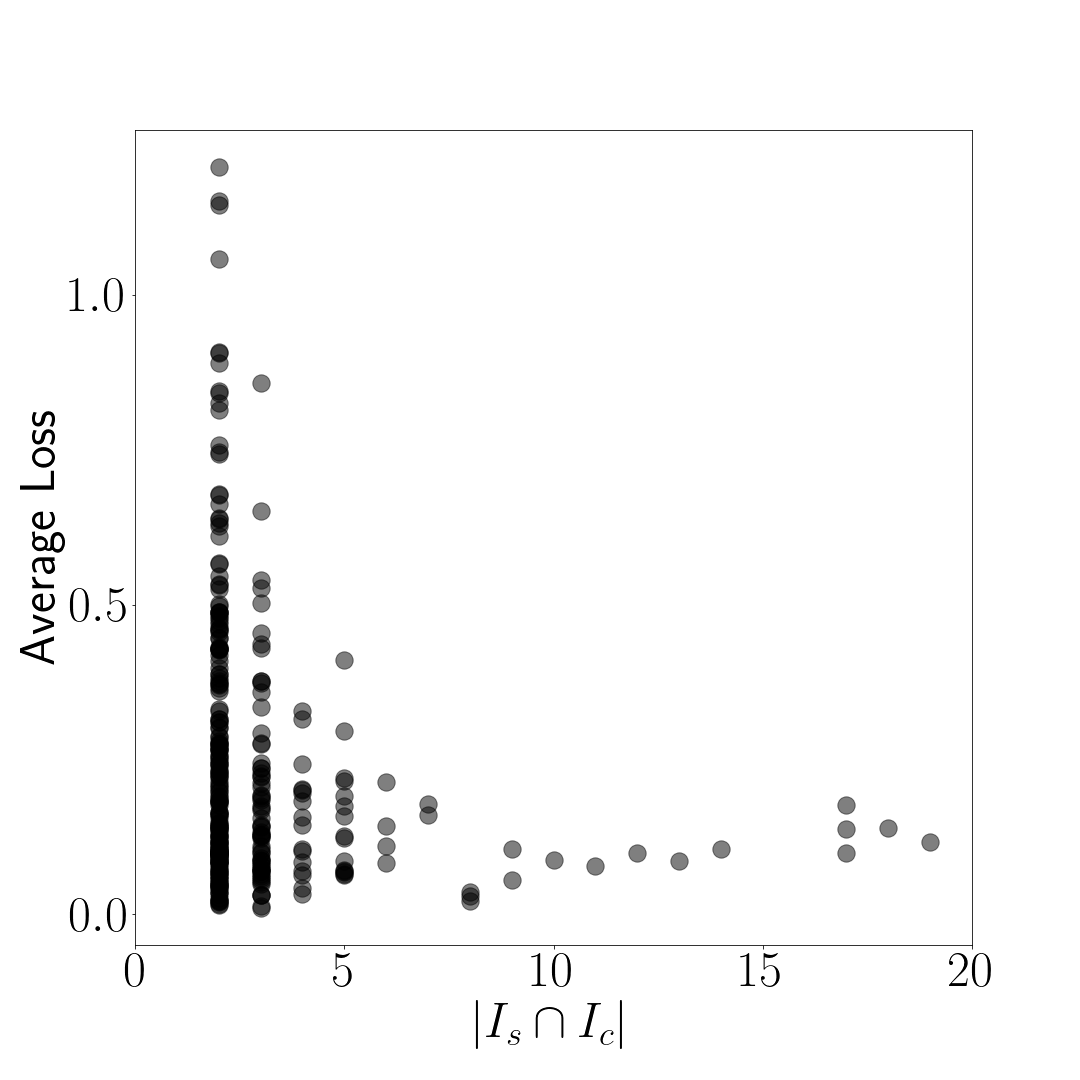
\includegraphics[width=0.3\textwidth]{figs/losssummary.png}
}}
\caption{\ref{fig:losssummary} Losses from leave-one-out cross-validation of candidate models.
\textbf{Bold} numbers are best for their major structure.
\ref{tab:losssummary} Empirical performance of selected EL model by data abundance.
The model is more accurate in Cre-leaf combinations where it draws on more data.}
\end{table}

\subsection{Connectivities}

Our main result is the estimation of matrices $\hat {\mathcal C}_v \in \mathbb R_{\geq 0}^{S \times T}$ representing connections of source structures to target structures for particular Cre-lines $v$. 
We confirm the detection of several well-established connectivities within our tensor, although we expect additional interesting biological processes to be identifiable.
The connectivity tensor and code to reproduce it are available at \url{https://github.com/AllenInstitute/mouse_connectivity_models/tree/2020}.

\subsubsection{Overall connectivity}

Several known biological projection patterns are evident in the wild-type connectivity matrix $\mathcal C_{wt}$ shown in Figure \ref{fig:full_wt}.
This matrix shows connectivity from leaf sources to leaf targets.
Large-scale patterns like intraareal connectivities and ipsilateral connections between cortex and thalumus are clear, as in previous estimates in \citet{Oh2014-kh, Knox2019-ot, Harris2019-mr}.

The layer-specific targeting of the different Cre-lines enables our estimated wild-type connectivities to resolve at the layer level.
This contrasts the model in \citet{Knox2019-ot}, which is denominated as the NW Major-WT model whose accuracy is evaluated in Table \ref{tab:crossvalidation}.
Layer-specificity is a major advantage of including distinct Cre-lines.
For comparison, we also plot averages over component layers weighted by layer size projections between summary-structure sources and targets in the cortex in Figure \ref{fig:cortex_wt}.
Our connectivities therefore exhibit a finer differentiation between regions than those in \citet{Knox2019-ot}
This also enables us to lower our limit of detection and examine a broader range of connectivity strengths.
Importantly, as shown in Table \ref{tab:crossvalidation} this finer spatial resolution corresponds to the increased accuracy of our EL model over the NW Major-WT model.

\newpage

\begin{figure}[H]
\centering
    \subfloat[] {
    \label{fig:full_wt}
    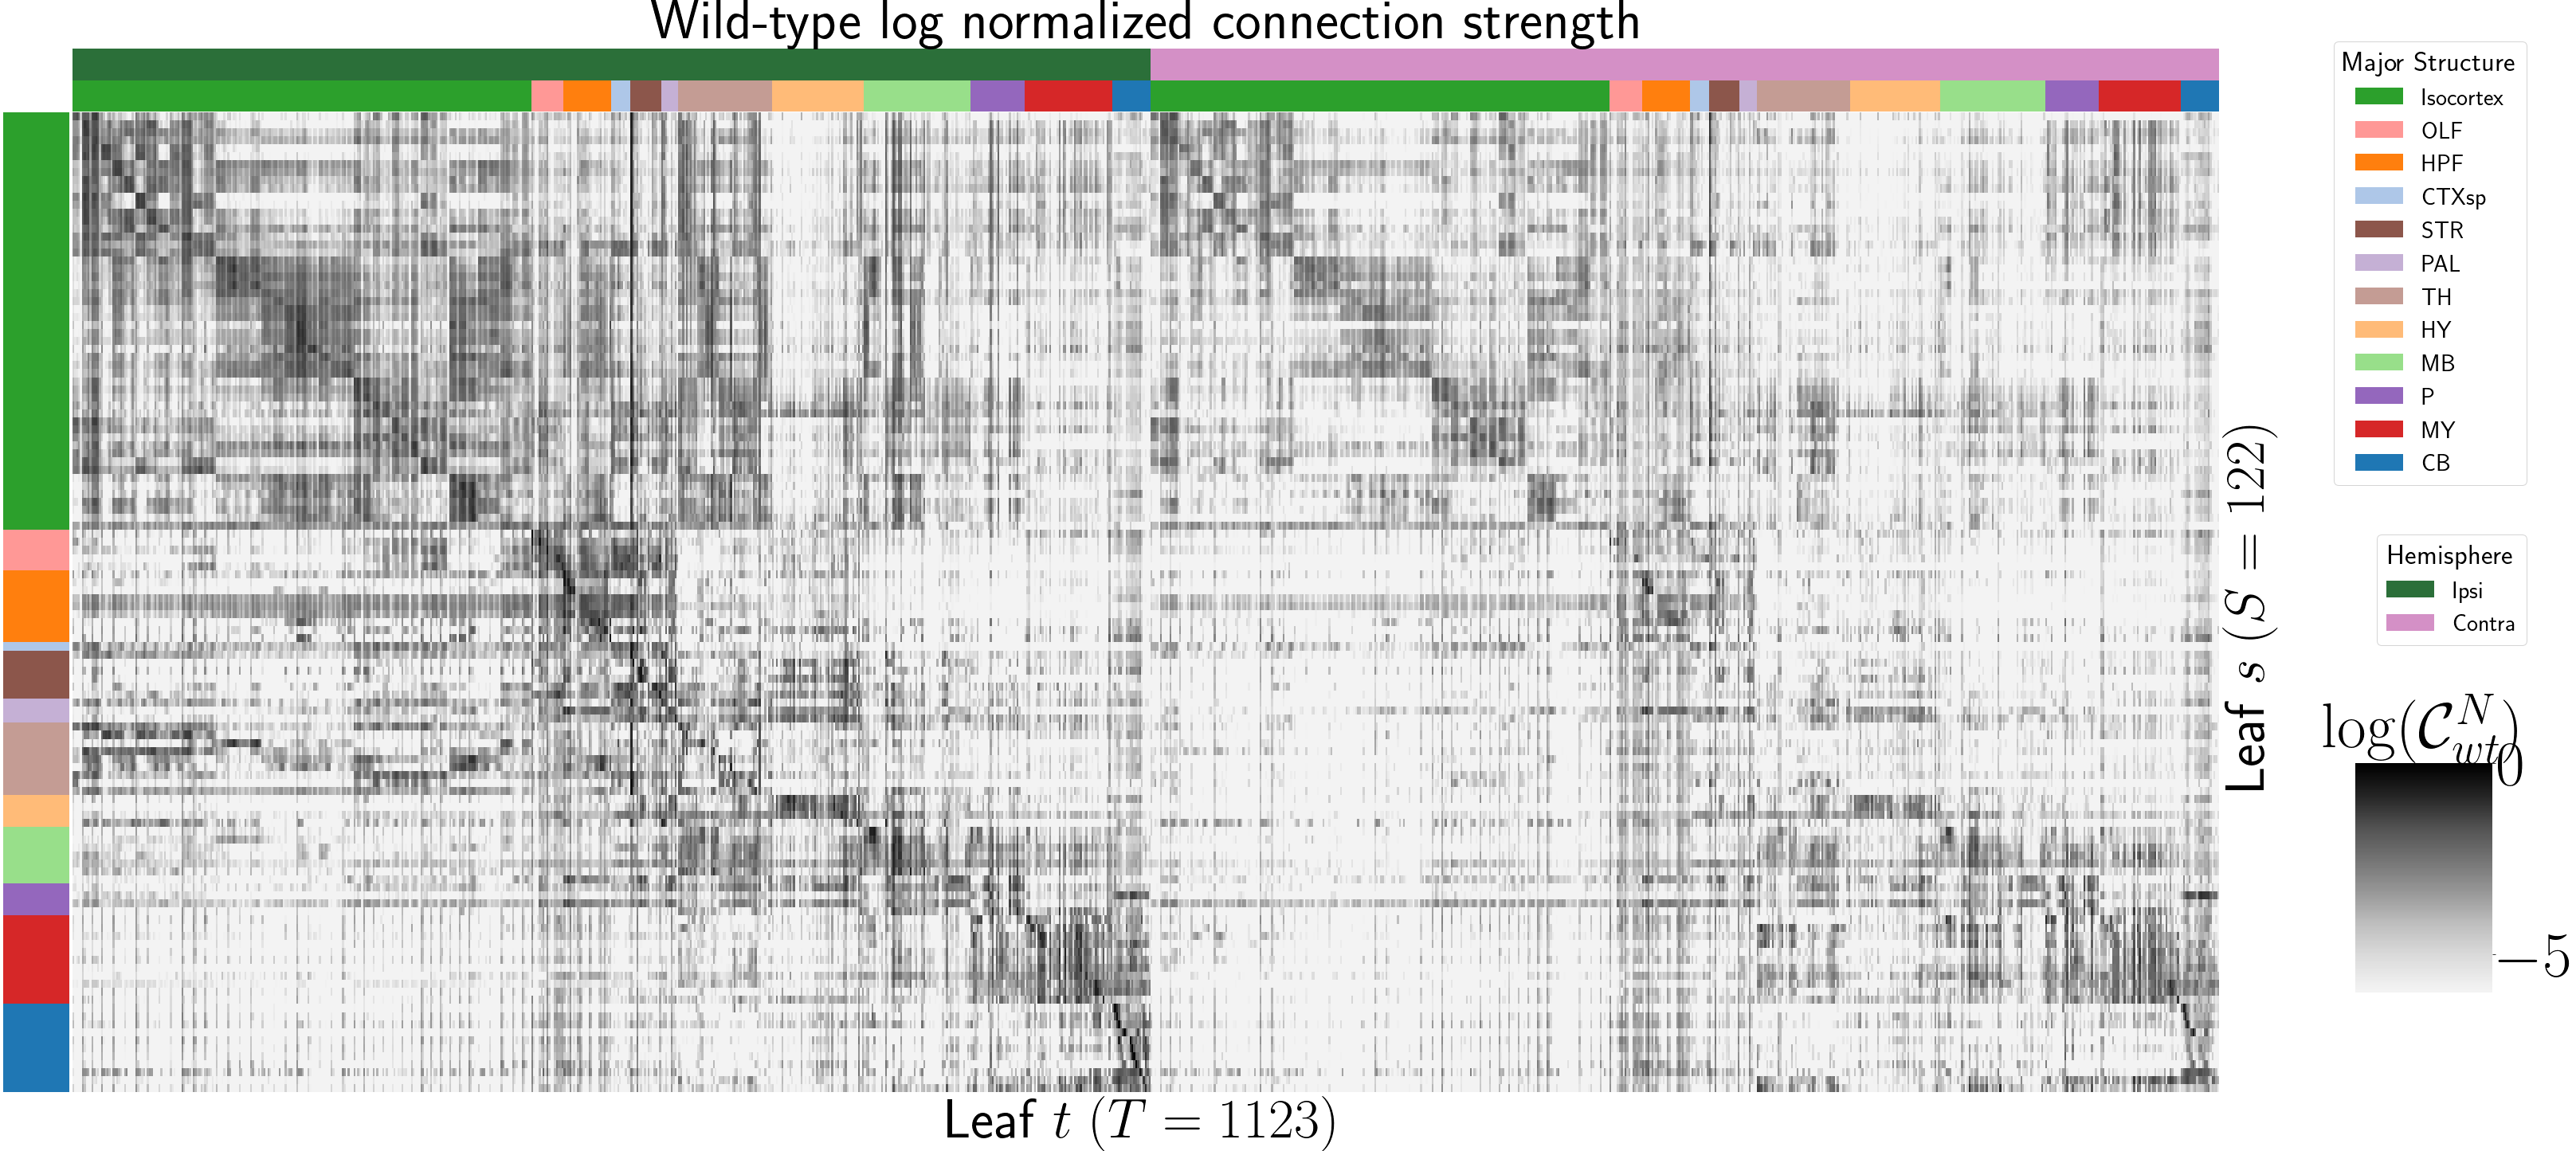
\includegraphics[width = \textwidth]{figs/conn_leaf2.png}
    } 
        \newline
       \subfloat[] {
    \label{fig:cortex_wt}
    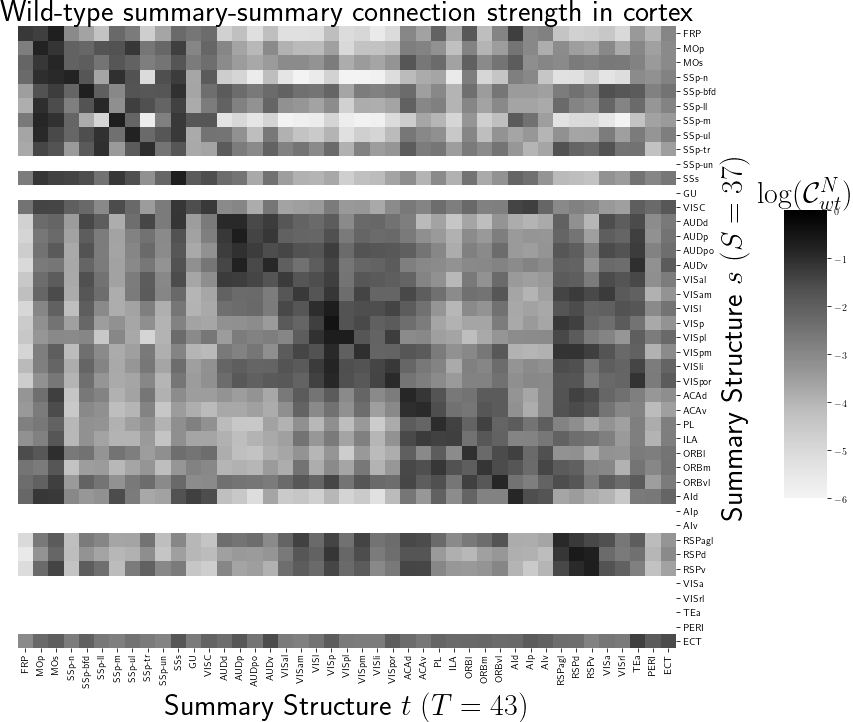
\includegraphics[width = .5\textwidth]{figs/conn_sum_cortex.png}
    } 
   \caption{Wild-type connectivities.
   \ref{fig:full_wt} Log wild-type connectivity matrix $\log \mathcal {C} (s,t,v_{wt})$.
   \ref{fig:cortex_wt} Log wild-type intracortical connectivity matrix at the summary structure level.}
   \label{fig:connectome}
\end{figure}

\newpage
\subsubsection{Class-specific connectivities}

Since source and cell-type combinations which project similarly indicate the network structure underpinning cognition, we investigate the presence of several biological processes within our connectivity estimates.
Although there is a rich anatomical literature using anterograde tracing data to describe projection patterns from subcortical sources to a small set of targets of interest, much of the accessible whole brain projection data is from the MCA project used here to generate the connectome models.
Thus, to validate our results while avoiding a circular validation of the data used to generate the model weights, we confirm that these class-specific connectivities exhibit certain known behaviors.
The cell types and source areas with extensive previous anatomical descriptions of projections using both bulk tracer methods with cell type specificity and single cell reconstructions that we investigate are 1) thalamic-projecting neurons in the visual and motor cortical regions, 2) cholinergic neurons in the medial septum and nucleus of the diagonal band (MS/NDB);
%3) cholinergic neurons in the caudoputamen,
and 3) serotonergic neurons of the dorsal raphe nucleus (DR).
Our estimated connections are in agreement with literature on these cell types.

\paragraph{Dependence of thalamic connection on cortical layer.}

Visual cortical areas VISp and VISl and cortical motor areas MOp and MOs have established layer-specific projection patterns that can be labeled with the layer-specific Cre-lines from the Allen datasets and others \citet{Jeong2016-dc, Harris2019-mr}.
Figure \ref{fig:ct_spc} shows that in VISp, the Ntsr1-Cre line strongly targets the core part of the thalamic LGd nucleus while in VISl, it a strong projection to the LP nucleus.
In VISp, the Rbp4-Cre line strongly targets LP as well.  
Rbp4-Cre and Ntsr1-Cre injections target layers 5 and 6 respectively.
Since we only generate connectivity estimates for structures with at least one injection centroid, this is shown by the position of non-zero rows in Figure \ref{fig:ct_spc}.
To fill these gaps, as a heuristic alternative model, we also display an average connectivity matrix over all Cre-lines.

\paragraph{MS and NDB projections in the Chat-IRES-Cre-neo model.}

Cholinergic neurons in the MS and NDB are well-known to strongly innervate the hippocampus, olfactory bulb, piriform cortex, entorhinal cortex, and lateral hypothalamus \citep{Zaborszky2015-fm, Watson2012TheMN}.
In the Allen MCA, cholinergic neurons were labeled by injections into Chat-IRES-Cre-neo mice.
Figure \ref{fig:cholinergic} checks the estimated connectome weights to targets in these major brain divisions from MS and NDB.
We observed that all these expected divisions were represented above the 90th percentile of weights from these source structures.

We also compared our Chat-IRES-Cre connectome model data for MS and NDB with the targets identified by  \citet{Li2018-nu}.
This single cell whole brain mapping project using Chat-Cre mice fully reconstructed n=50 cells to reveal these same major targets and also naming additional targets from MS/NDB \citep{Li2018-nu}.
We identified ~150 targets at the fine leaf structure level among the top decile of estimated weights.
To directly compare our data across studies, we merged structures as needed to get to the same ontology level, and remove ipsilateral and contralateral information.
After formatting our data, we found 51 targets in the top 10\%; Li et al. reported 47 targets across the 50 cells.
There was good consistency overall between the target sets; 35 targets were shared, 12 were unique to the single cell dataset, and 16 unique to our model data.
We checked whether targets missing from our dataset were because of the threshold level.
Indeed, lowering the threshold to the 75 th percentile confirmed 6 more targets-in-common, and all but 2 targets from \citet{ Li2018-nu} were above the 50th percentile weights in our model.
Of note, the absence of a target in the single cell dataset that was identified in our model data is most likely due to the sparse sampling of all possible projections from only n=50 MS/NDB cells.

%\paragraph{CP projections in the Chat-IRES-Cre-neo model.}
%Most cells in the caudoputamen (CP) are GABAergic spiny projection neurons.
%These cells are also the only type that send projections outside the CP.
%Cholinergic interneurons make up 1-2\% of all CP cells and their axon terminals do not extend beyond the CP borders.
%We confirmed that the model predictions for connection weights from CP cholinergic cells were consistent with this known anatomy; the connection weight to CP was $\sim2$-fold higher than any other in the top $5\%$.

\paragraph{DR projections in the Slc6a4-Cre\_ET33 model.}

Serotonergic projections from cells in the dorsal raphe (DR) are widely distributed and innervate many forebrain structures including isocortex and amygdala.
In the Allen MCA, serotonergic neurons were labeled using Slc6a4-Cre\_ET33 and Slc6a4-CreERT2\_EZ13 mice.
This small nucleus appears to contain a complex mix of molecularly distinct serotonergic neuron subtypes with some hints of subtype-specific projection patterns \citep{Ren2018-ty, Ren2019-jg,  Huang2019-xh}.
We expect that the Cre-lines used here in the Allen MCA, which use the serotonin transporter promoter (Slc6a4-Cre and -CreERT2), will lead to expression of tracer in all the serotonergic subtypes recently described in an unbiased way, but this assumption has not been tested directly.
We compared our model data to a single cell reconstruction dataset consisting of n=50 serotonergic cells with somas in the DR that also had bulk tracer validation \ref{fig:serotinergic}.
After processing our data to match the target structure ontology level across studies, we identified 37 targets from the DR with weights above the 90th percentile, whereas \citet{ Ren2019-jg} listed 55 targets across the single cell reconstructions.
Twenty seven of these targets where shared.

Overall there was good consistency between targets in olfactory areas, cortical subplate, CP, ACB and amygdala areas, as well in palidum and midbrain, while the two major brain divisions with the least number of matches are the isocortex and thalamus.
There are a few likely reasons for these observations.
First, in the isocortex, there is known to be significant variation in the density of projections across different locations, with the strongest innervation in lateral and frontal orbital cortices \citet{ Ren2019-jg,}. %e.g., see MCA experiment 480074702 and Figs. 6, 7 in Ren 2019
Indeed, when we lower the threshold and check for weights of the targets outside of the 90\%, we see all but one of these regions (PTLp, parietal cortex which is not frontal or lateral) has a weight assigned in the top half of all targets.
In the thalamus, our model predicted strong connections to several medial thalamic nuclei (i.e., MD, SMT) that were not targeted by the single cells.
This discrepancy may be at least partially explained by the complex topographical organization of the DR that, like the molecular subtypes, is not yet completely understood.
A previous bulk tracer study that specifically targeted injections to the central, lateral wings, and dorsal subregions of the DR reported semi-quantitative differences in projection patterns \citep{Muzerelle2016-sn}.%( Muzarelle et al. 2016% , Table 3).
Notably, \citet{Muzerelle2016-sn} report that cells in the ventral region of DR project more strongly to medial thalamic nuclei, whereas the lateral and dorsal DR cells innervate more lateral regions (e.g., LGd).
Thus, it is possible that the single cell somas did not adequately sample the entire DR.

\newpage

\begin{figure}[H]
\subfloat[]{
\label{fig:ct_spc}
    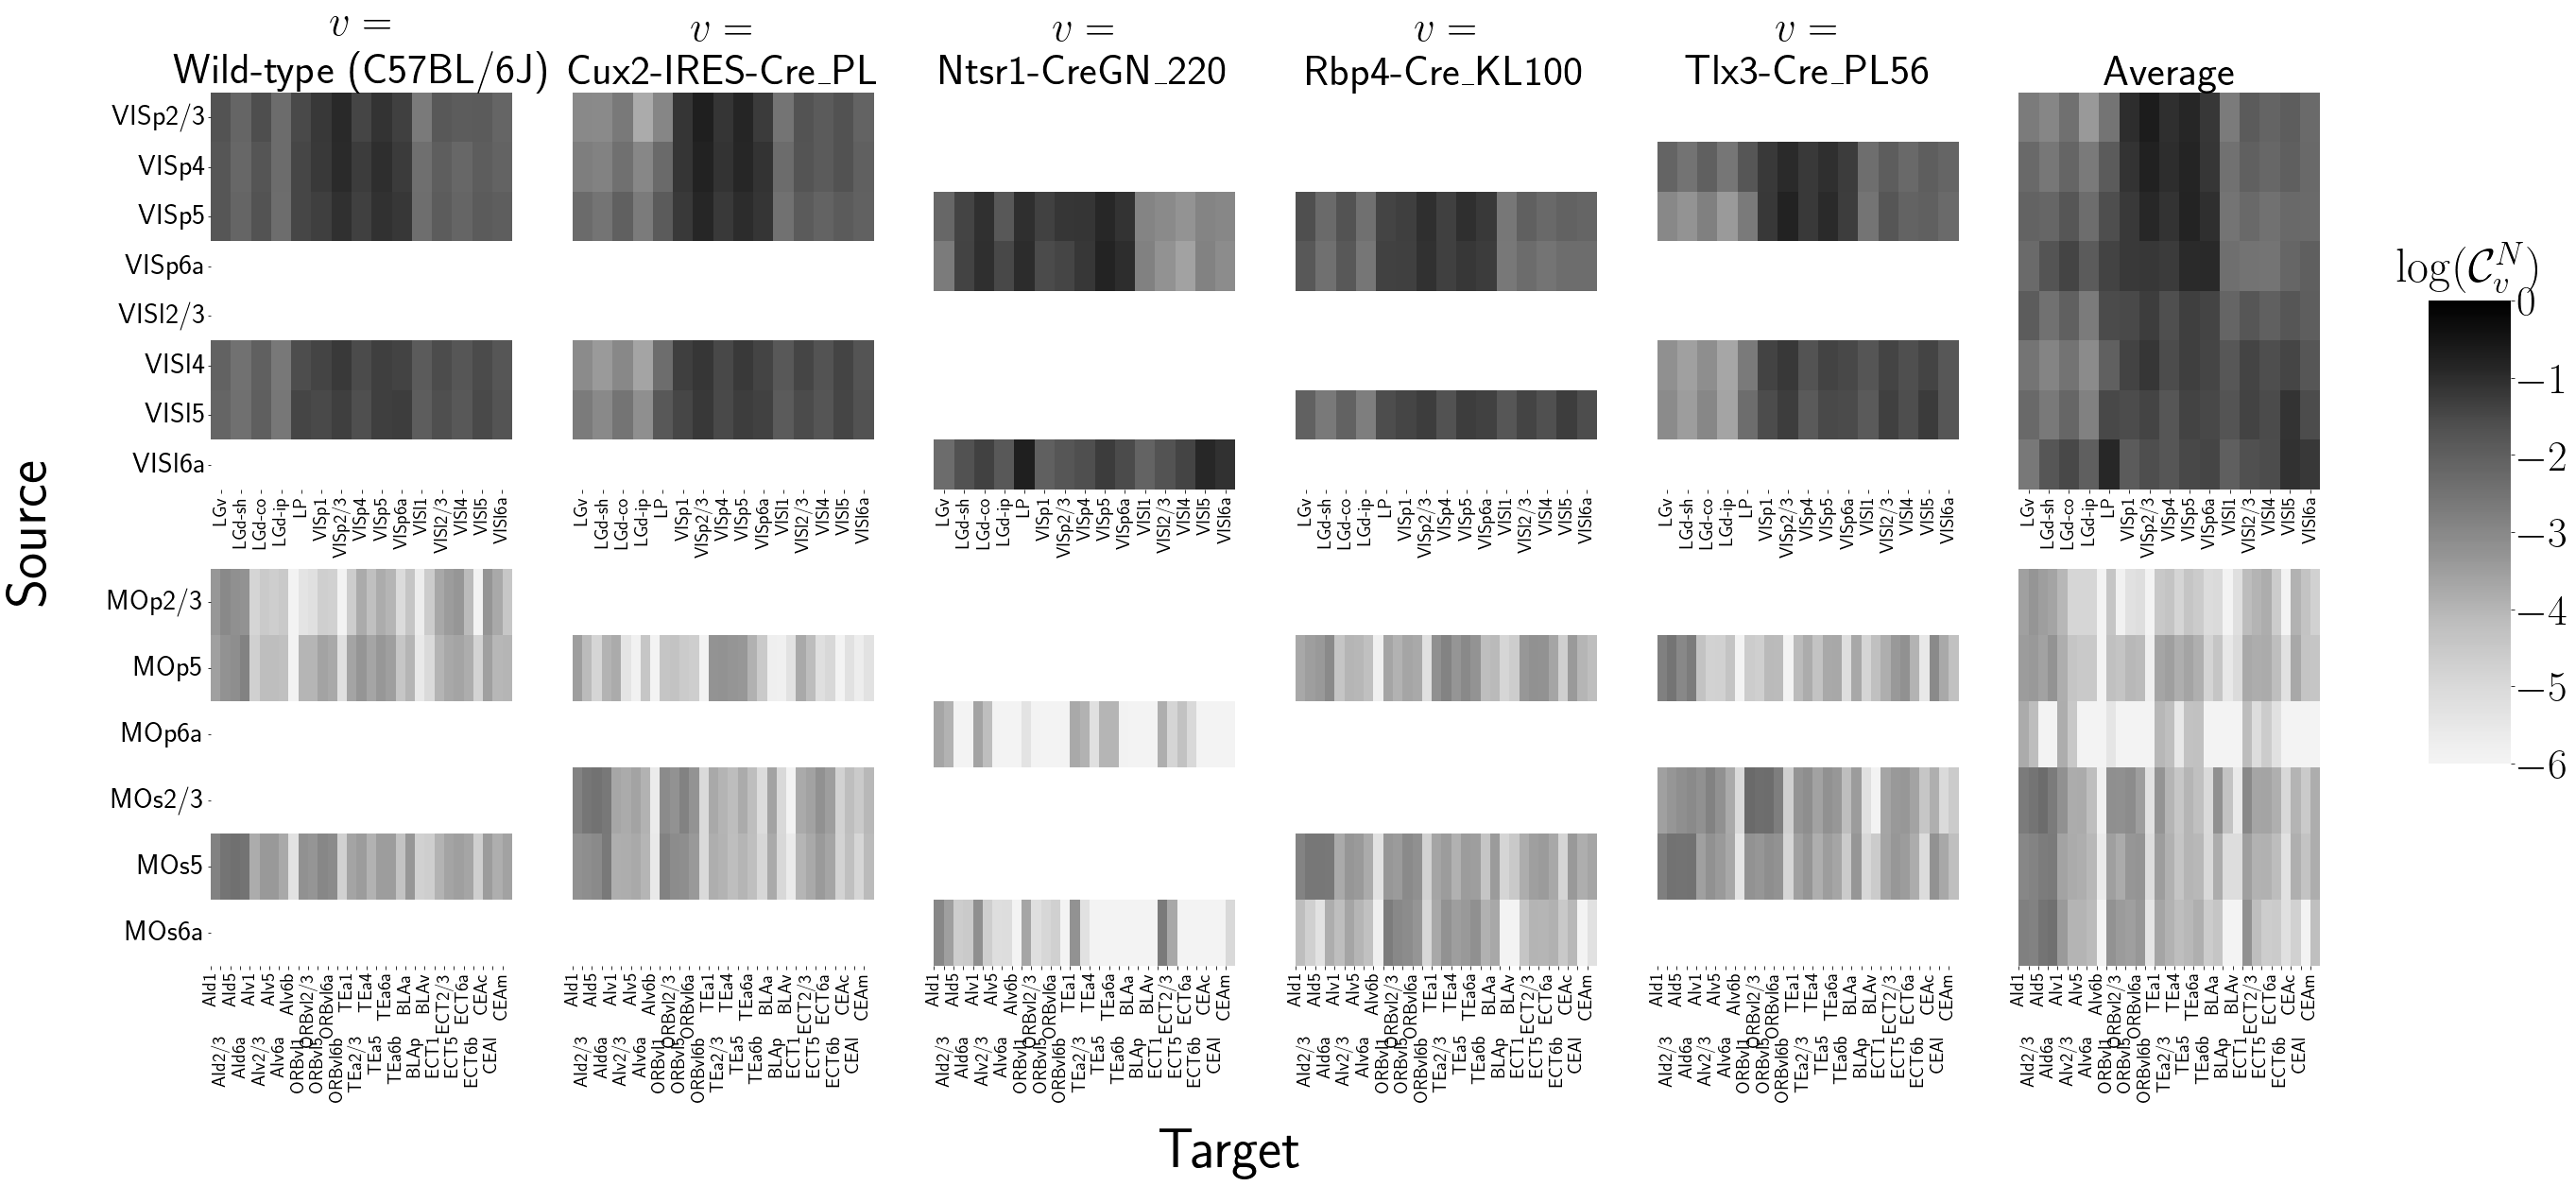
\includegraphics[width=.8\textwidth]{figs/visp_mo.png} 
    }
    \newline
 \subfloat[]{
 \label{fig:cholinergic}
    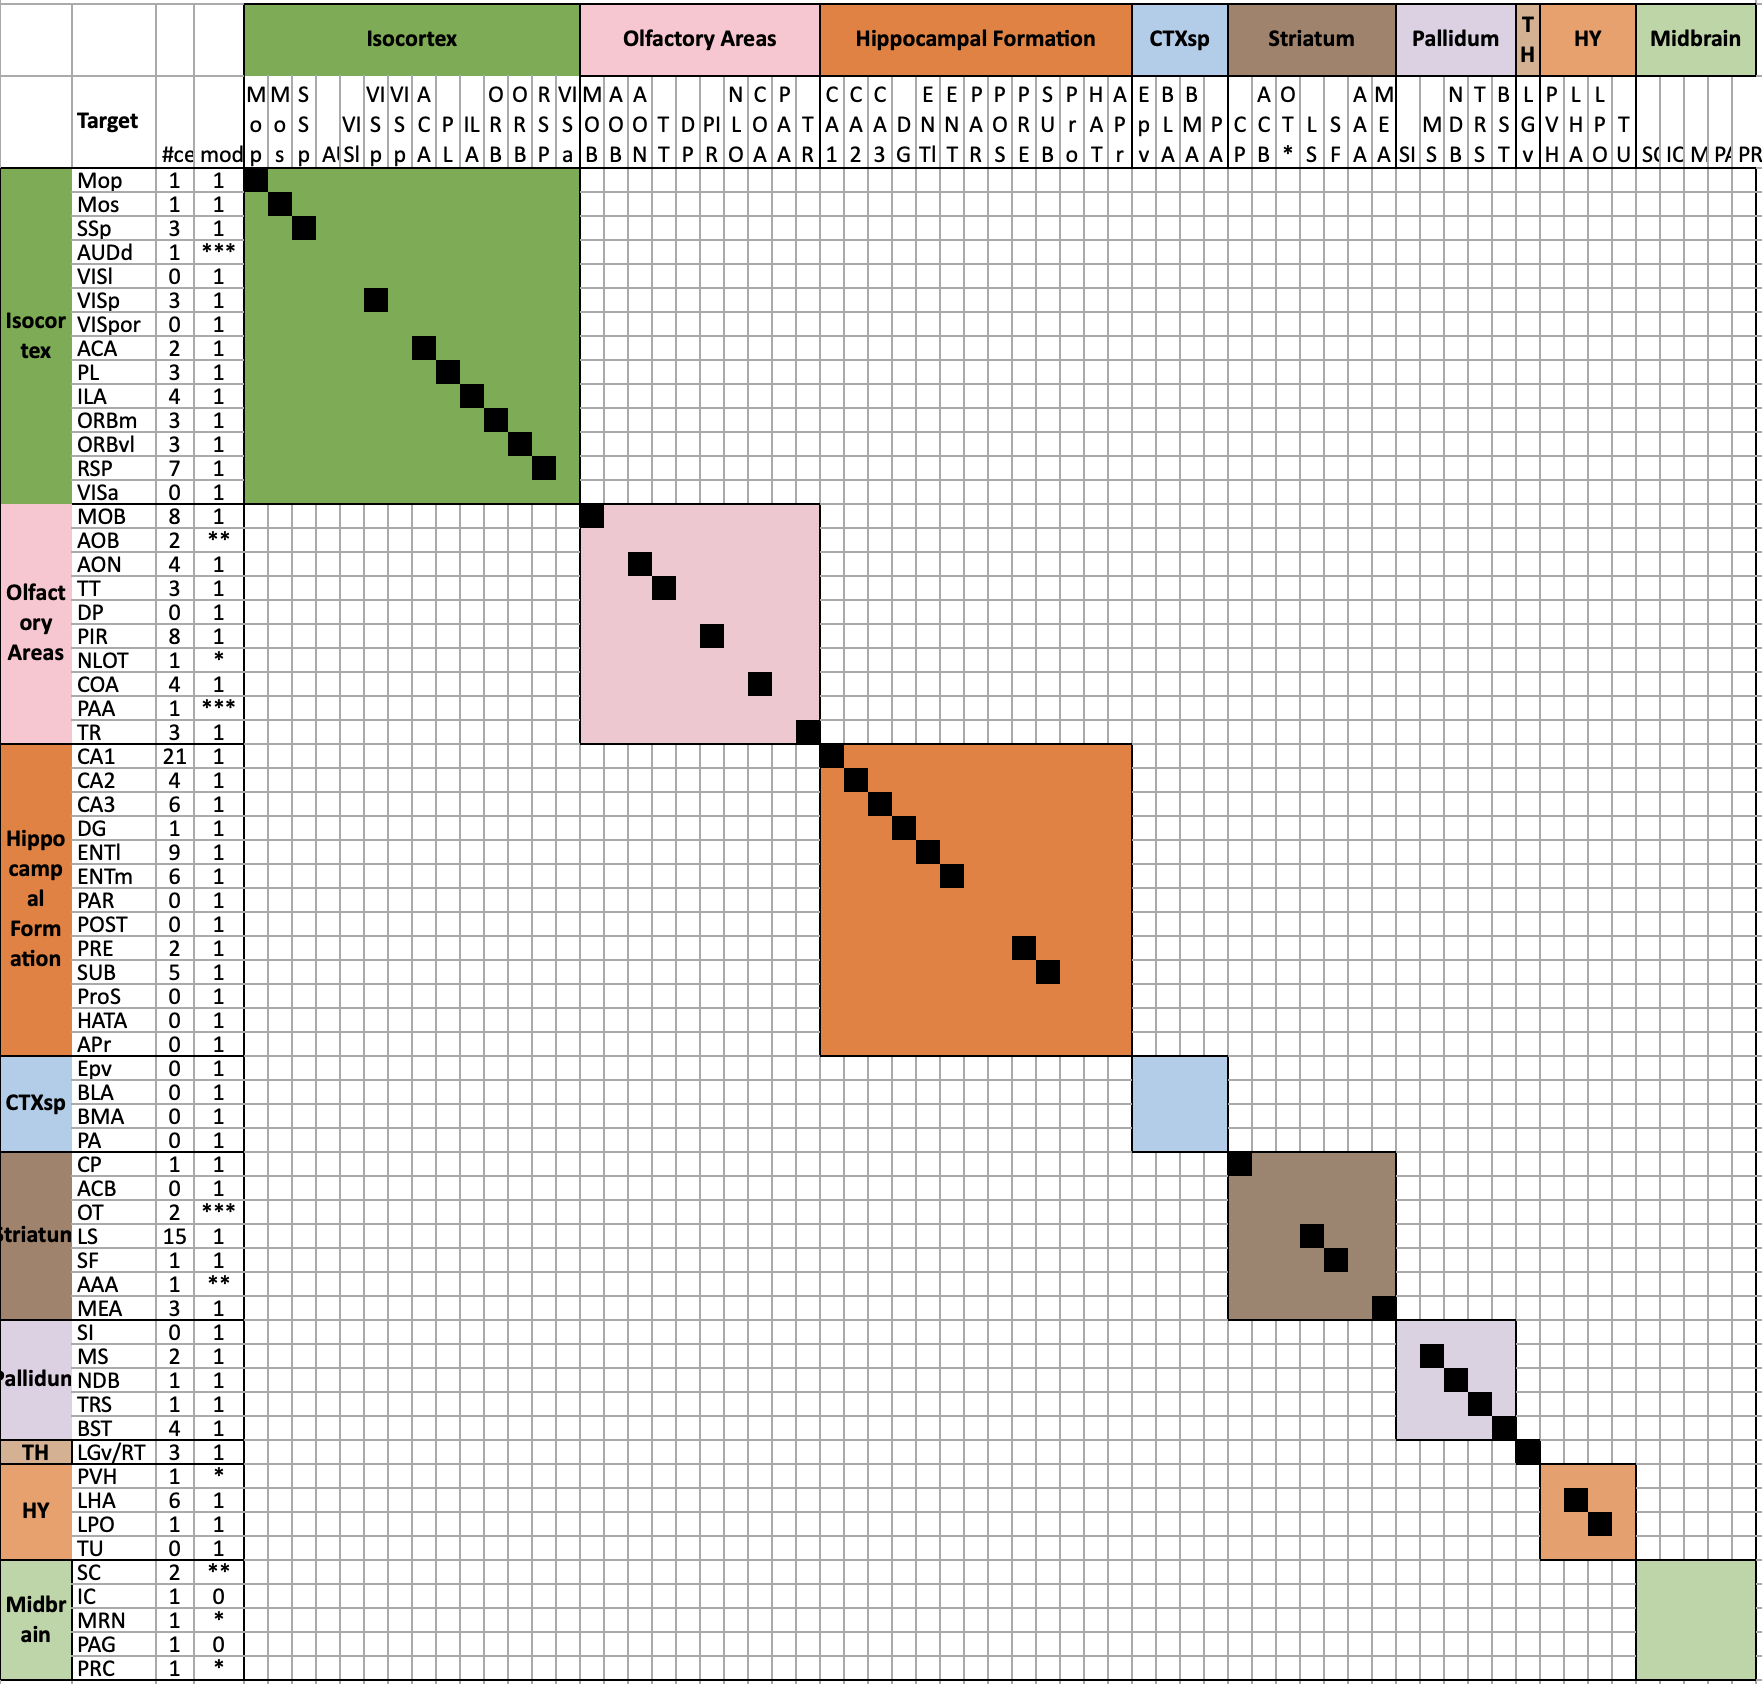
\includegraphics[width=.4\textwidth]{figs/cholinergic.png} 
    }
     \subfloat[]{
      \label{fig:serotinergic}
    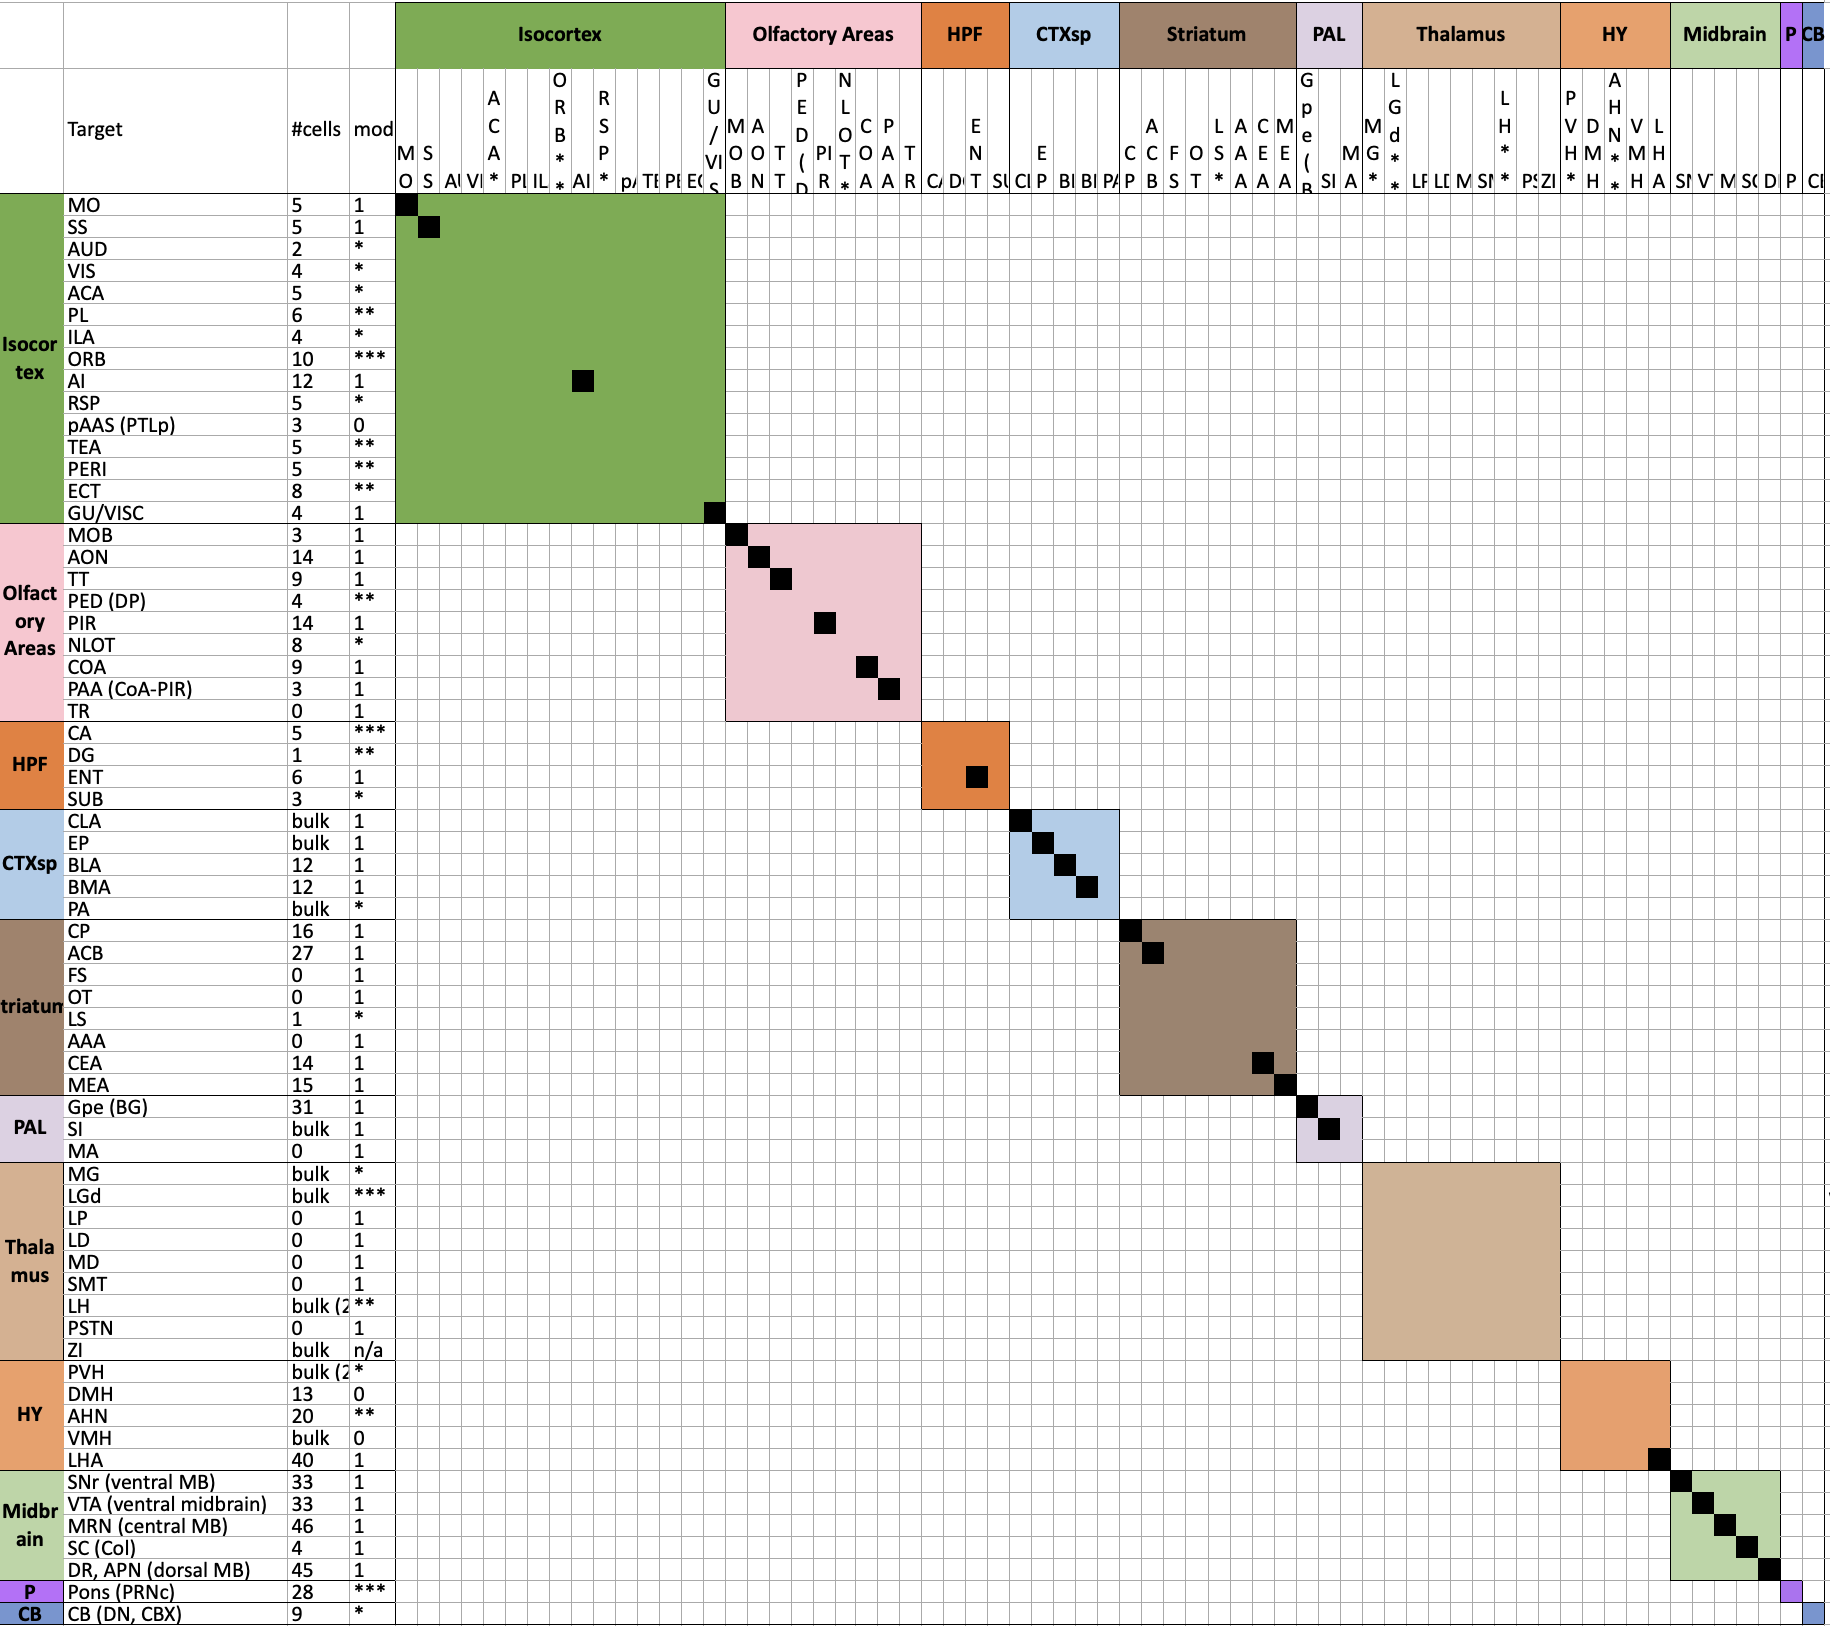
\includegraphics[width=.42\textwidth]{figs/serotinergic.png} 
    }
    \caption{  Cell-class specificity. \ref{fig:ct_spc} Selected cell-class and layer specific connectivities from two visual and two motor areas.
	 Sources without an injection in the Cre driver line are not estimated due to lack of data for that Cre-line in that structure.
	 \ref{fig:cholinergic} Targets reported for cholinergic cells in MS/NDB in \citet{ Li2018-nu}  and above the 90th percentile in our Chat-IRES-Cre-neo model.  A black box along the diagonal indicates the target was identified in both studies ($n=35$). The number of single cells (out of 50) with a projection to each target is shown in the first column after the target acronym and the next column shows whether a target appeared in the $90\%$ thresholded model weights (1= present, 0=absent). Some of these targets only appeared at lower thresholds as indicated by asterisks, $*** >85th \%, ** >75th \%, * >50th \%$.
\ref{fig:serotinergic} Targets reported for serotonergic cells in DR in \citet{Ren2018-ty, Ren2019-jg} and above the 90th percentile in our Slc6a4-Cre\_ET33 model.
    		}
\label{fig:data_ct}
\end{figure}

\newpage

\subsection{Connectivity Analyses}

Cell-classes exhibit a wide range of connectivities.
Figure \ref{fig:ct_clust} shows a collection of connectivity strengths generated using cre-specific models for wild-type, Cux2, Ntsr1, Rbp4, and Tlx3 cre-lines from VIS areas at leaf level in the cortex to cortical and thalamic nuclei.
%than summary structure especially when looking at targets at major brain division level.
We use hierarchical clustering to sort source structure/cell-class combinations by the similarity of their structural projections, and sort target structures by the structures from which they receive projections.
Examining the former, we can see that the layer 6 Ntsr1 Cre-line distinctly projects to thalamic nuclei, regardless of source summary structure.
This contrasts with the tendency of other cell-classes to project intracortically in a manner determined by the source structure.
Similarly, layer 6 targets are not strongly projected to by any of the displayed cell classes.
%There are too many targeted summary structures to plot here, but we expect that the source profile of each target clusters by structure.

This exploratory analysis lead us to investigate matrix decomposition methods for our estimated connectivity matrices.
We applied non-negative matrix factorization to decompose the long-range wild-type connectivities into linear combinations of learned latent connectivities.
In particular, we censor short range connections due to their clear biological derivation from diffusion and their high mathematical rank.
This decomposes the remaining censored connectivity matrix into a linear model based off a relatively small number of distinct signals.

In contrast to the complex tree of cell types implied by heirarchical clustering, this creates a simple linear statistical model of overall connectivity. \skcomment{citation}
These signals are plotted in Figure \ref{fig:nmf_results}, and technical details and results are given in Supplemental Sections \ref{supp_sec:matrix_factor_methods} and \ref{supp_sec:matrix_factor_results}, respectively.
Connectivity patterns like cortical-cortical and cortical-thalamic are visible in this matrix factorization.
It generates a reconstructured connectivity matrix with structure and layer-specific targeting from a relatively small number of learned additive factors.
Supplemental Section \ref{supp_sec:matrix_factor_results} contains quantitative performance of this model, as well as association of factors in this model with individual Cre-lines.

%These details include a cross-validation based method for selecting the number of components, a masking method for focusing only on long range connections, and a stability method for ensuring that the decomposition is reliable across computational replicates.
%The plotted decomposition shows that these underlying connectivity archetypes correspond strongly to major brain division in both target and sources.
%However, certain components that predominantly represent connectivity from a given major brain division may also be accessed from other areas.
%For example, the IP and FN regions of CB are strongly associated in \ref{fig:W} with the component projecting to MY in \ref{fig:H}.

%Inspection of the reconstructed distal normalized connection strength using the top $15$ components shows qualitatively shows that this relatively sparse decomposition is able to capture much of the observed variability.
%Layer-specific targeting is evident, indicating that the factorization method is detecting cell-type specific signals, even though it is trained only on the wild-type connectivity.
%Other 

\newpage

\begin{figure}[H]
\centering
\hspace{1cm}
\subfloat[]{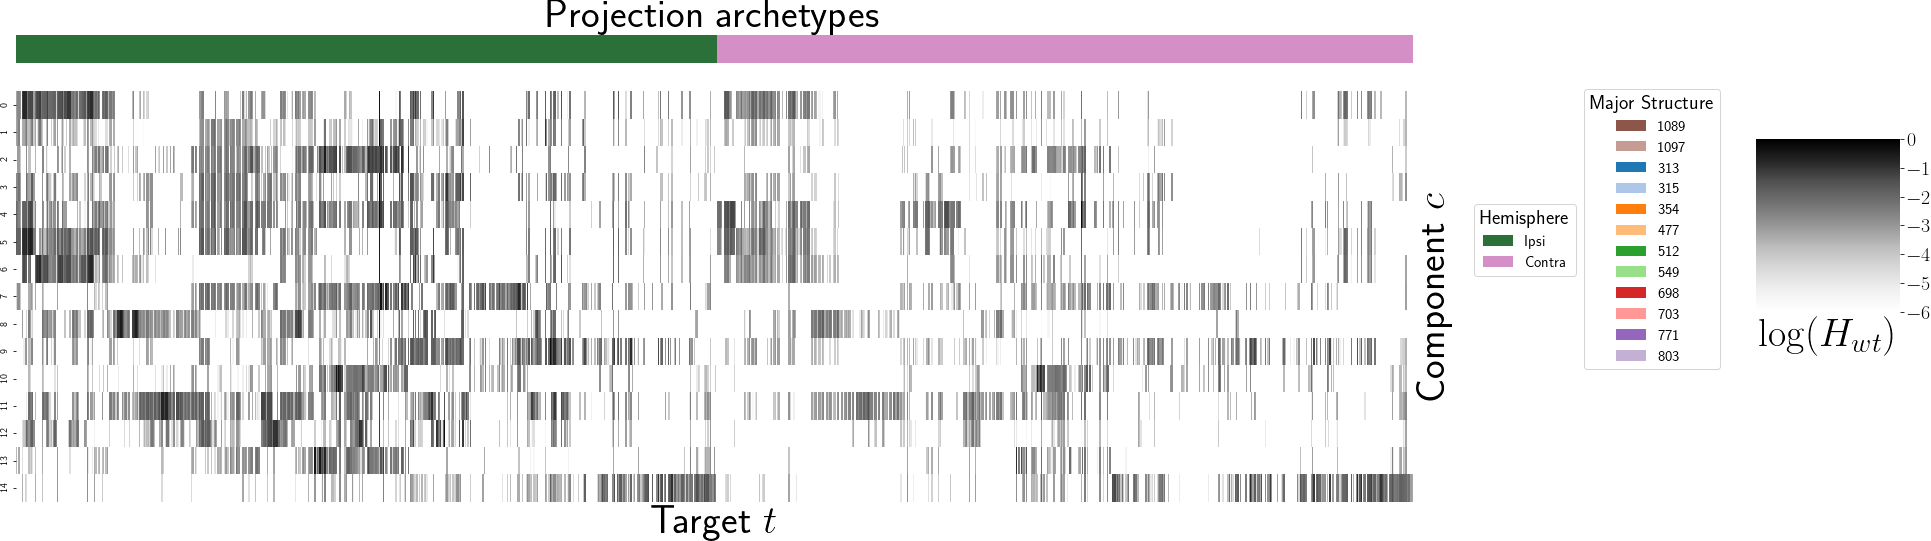
\includegraphics[width = .85 \textwidth]{figs/H_wt.png}
\label{fig:H}} 
\newline
\begin{tabular}[t]{cc}
\adjustbox{valign=t}{\subfloat[]{
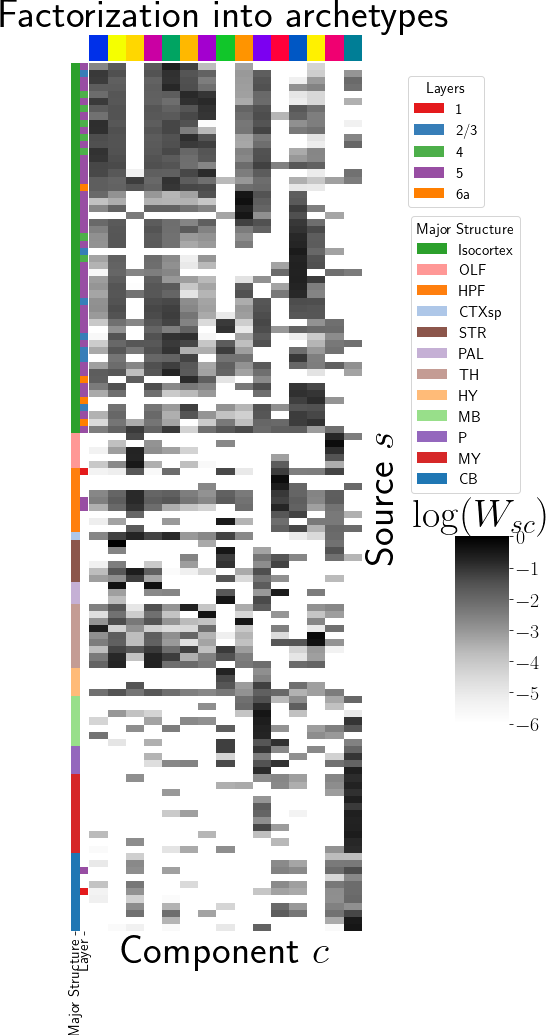
\includegraphics[width = .28\textwidth]{figs/W_wt.png}
\label{fig:W}}
} & 
\adjustbox{valign=t}{\subfloat[]{
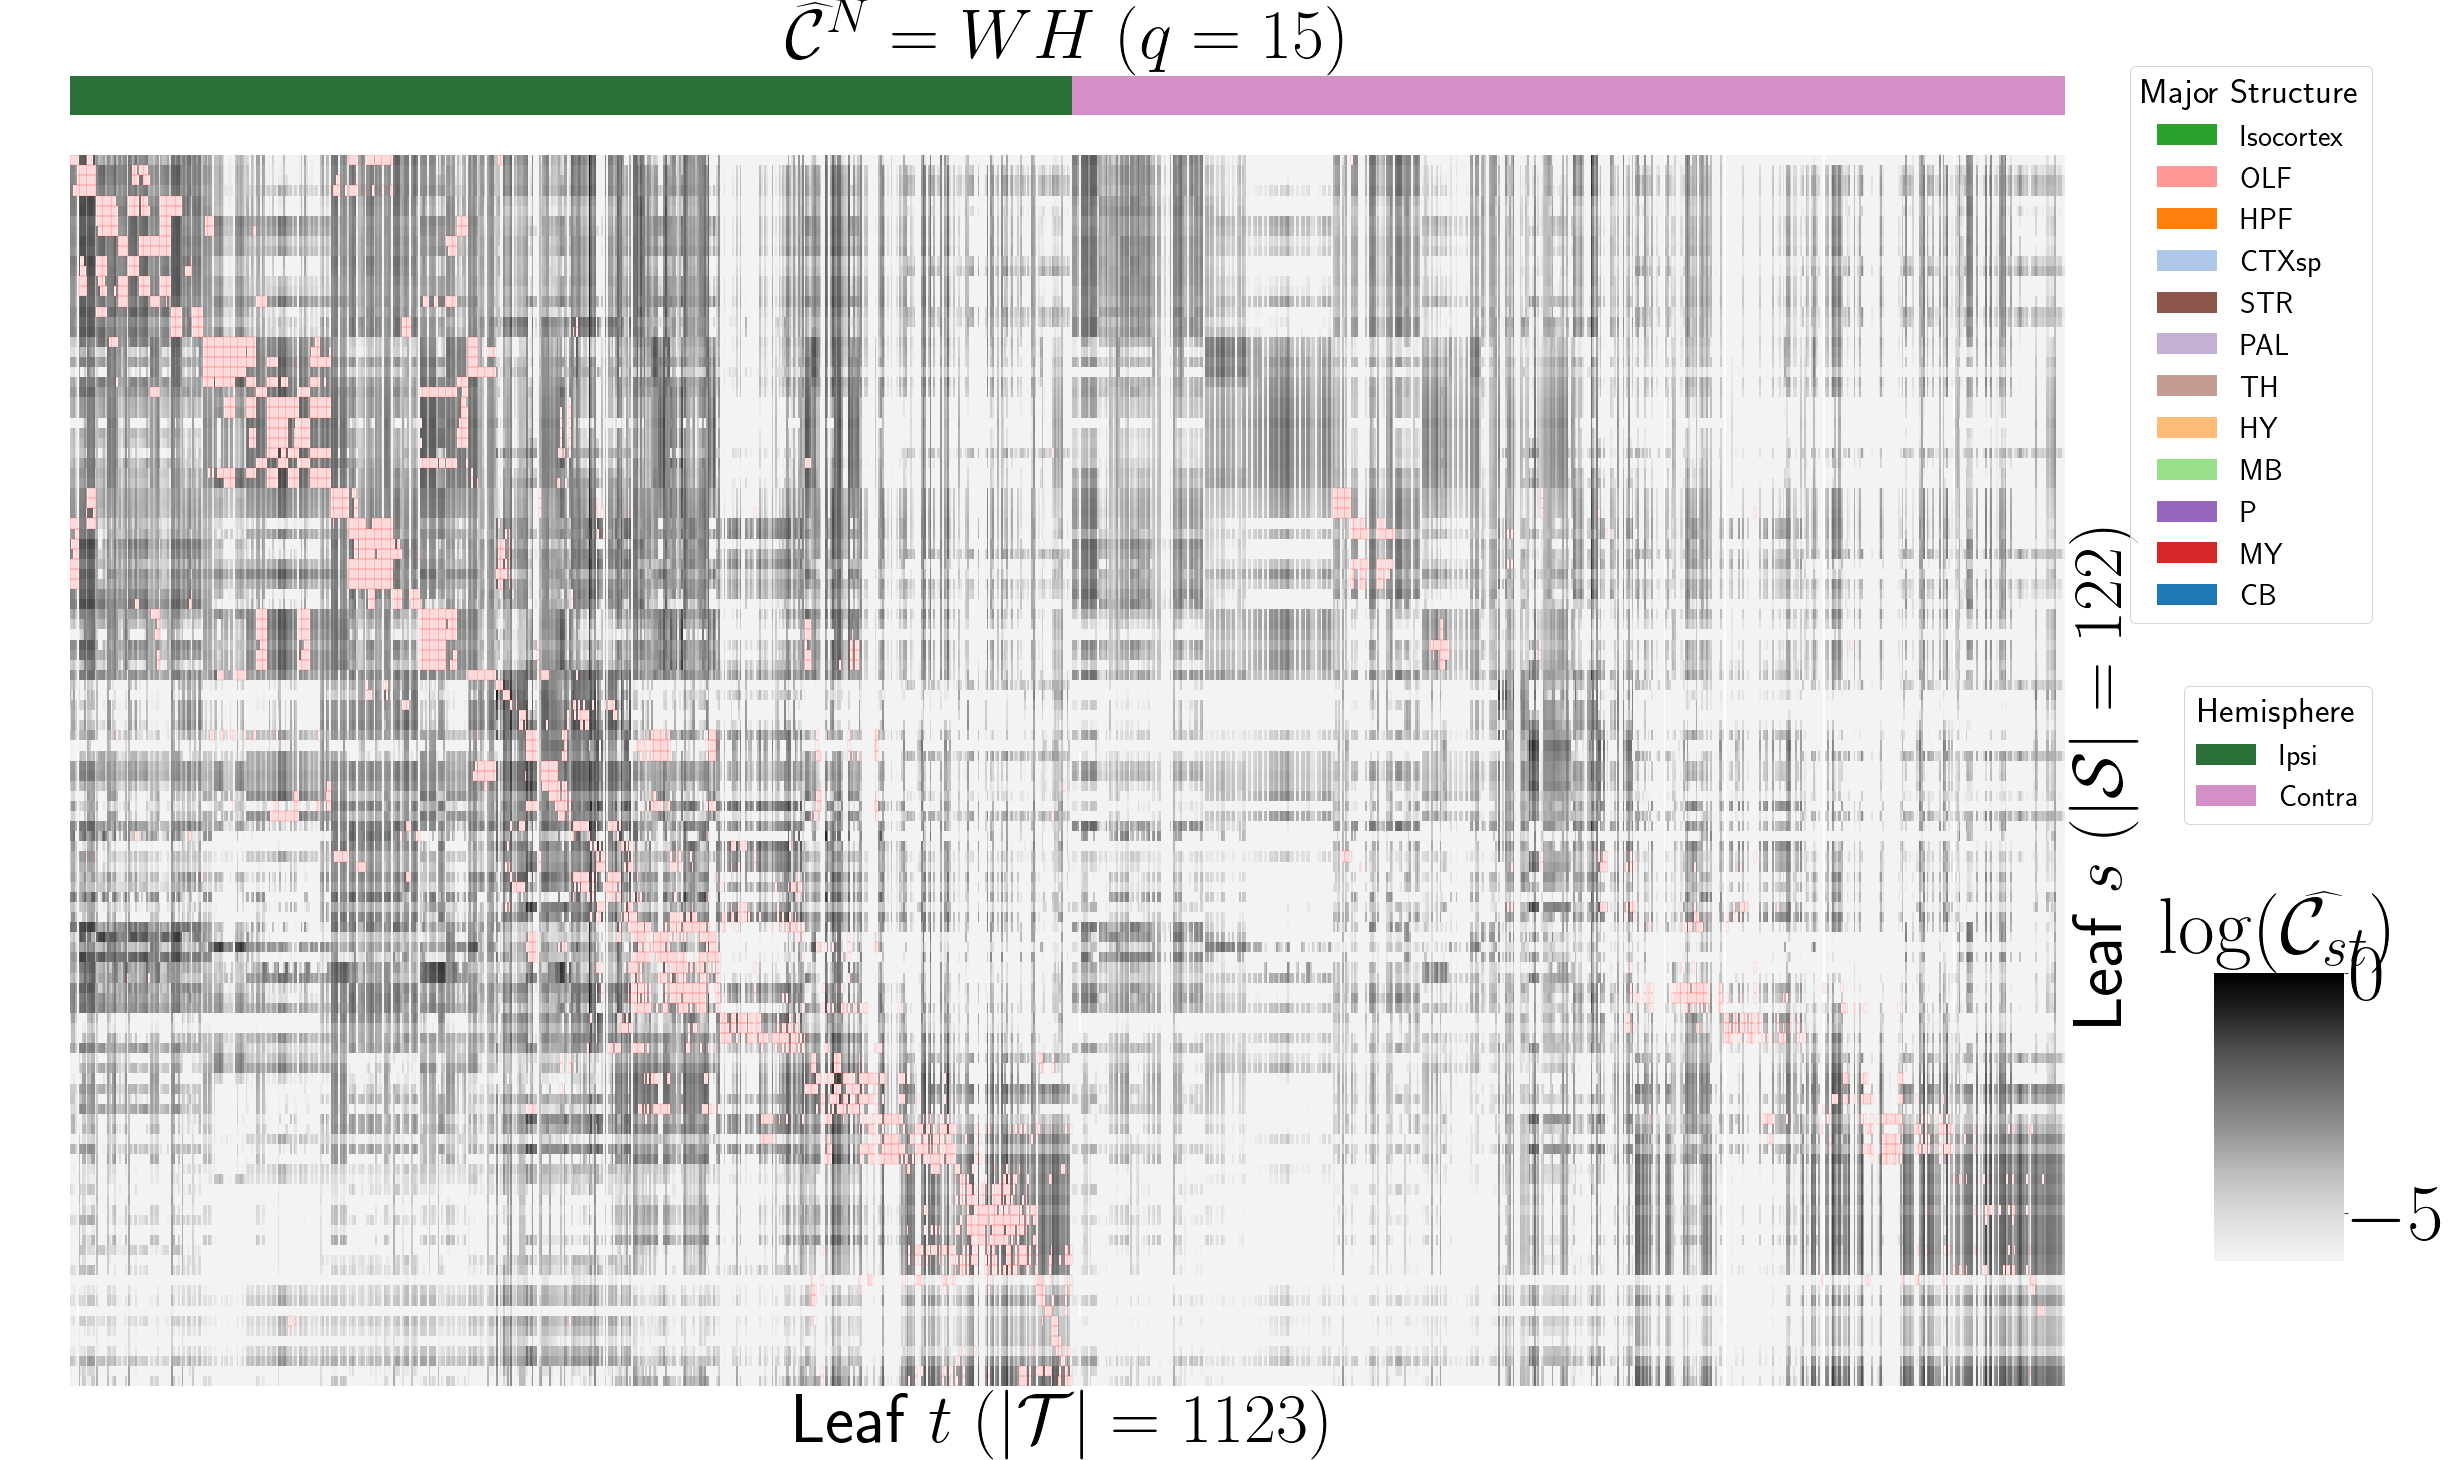
\includegraphics[width = .6\textwidth]{figs/conn_leafs_recon.png}
\label{fig:recon}}
} 
\end{tabular}
\caption{Non-negative matrix factorization results $\mathcal C_{wt}^N = WH$ for $q = 15$ components.
\ref{fig:H} Latent space coordinates $H$ of $\mathcal C$.
Target major structure and hemisphere are plotted.
\ref{fig:W} Loading matrix $W$.
Source major structure and layer are plotted.
\ref{fig:recon} Reconstruction of the normalized distal connectivity strength using the top $15$ archetypes.  Areas less than $1500 \mu m$ apart are not modeled, and therefore shown in pink.
}
\label{fig:nmf_results}
\end{figure}

\newpage

